% !TEX root = seminararbeit.tex

\section{Implementation}
\label{implementation}

% TODO: put text here
In the following sections the technology that was eventually used to implement \gls{SceGraToo} is dissected and explained in detail.

\subsection{Server}

The server has a small interface, meaning it does not have a lot of routes it serves.
When it receives a \texttt{GET} request from a client it tries to match the request to one of its routes.
If no route matches it tries to find a static files that matches the requested route URL.
If it finds the file, the file is served to the client.
If not a 404 HTTP code is returned, which means \texttt{Not Found}.
A \texttt{POST} route also exists for uploading content.
\texttt{POST} and \texttt{GET} are different HTTP methods.
An HTTP request to the same route can happen via different methods to evoke different action from the server \cite{httpmethods}.

Some of the routes the server answers to are:

\begin{description*}
  \item[\texttt{POST} /projects/:project/src/:file]
    saving files being uploaded
  \item[\texttt{GET} /projects]
    return all projects on the server
  \item[\texttt{GET} /projects/:project]
    return all information for the project \texttt{:project}
\end{description*}

\subsection{Client}

The client uses to frameworks to solve different problems.
Angular is used for managing and organizing most of the application, while react is used for highly dynamic views, like the tree-view.

\subsubsection{Angular}
\label{angular}

AngularJS is used for:

\begin{itemize*}
  \item Bootstrapping the application
  \item Modularization
  \item Dependency management
  \item Resource management
  \item Routing
  \item Less dynamic views
\end{itemize*}

\paragraph{Bootstrapping}
\label{par:Bootstrapping and Routing}

Web applications need to be bootstrapped. There has to be one entry-point
for starting the the application. And this entry-point
needs to be called after all scripts, that are referenced in the \gls{HTML}
document, have been downloaded from the server. Angular accomplishes this by
subscribing to the \texttt{DOMContentLoaded} event. Angular will then look for
\gls{DOM} elements with an \texttt{ng-app} attribute. That attribute is set by the
developer and tells angular, that the corresponding DOM element is supposed to
contain an application and the application's name. The bootstrapping process is
described in Figure~\ref{fig:angularbootstrap}.

\begin{figure}
  \centering
  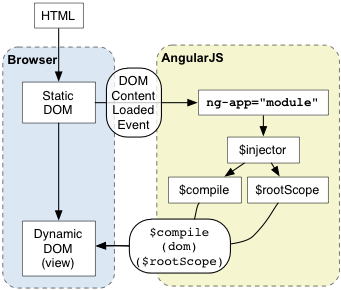
\includegraphics[width=0.5\textwidth]{../assets/concepts-startup.png}
  \caption{This is angulars bootstrapping process \cite{angularbootstrap}.}
  \label{fig:angularbootstrap}
\end{figure}

The code from Listing \ref{list:bootstrap} initializes SceGraToo. In the \texttt{config}
function, routes are defined. When a link is clicked, the browser will not issue a
request to the server and load that page. Instead, a new controller takes over and
renders a different template. The advantage of this approach is that the user
perceives immediate feedback, while navigating. The application can render the view and
react to user input, while it is still waiting for some requested resources from
the server (like a list of all available projects). This approach is called
single-page application \cite{Mikowski:2013:SPW:2663433}.

\begin{listing}
  \begin{minted}[breaklines,bgcolor=bg,linenos=true]{javascript}
window.angular.module('scegratooApp')
  .config(function ($routeProvider) {
    $routeProvider
      .when('/', {
        redirectTo: '/projects'
      })
      .when('/projects', {
        templateUrl: 'views/projects.html',
        controller: 'ProjectsCtrl'
      })
      .when('/projects/:project', {
        templateUrl: 'views/project.html',
        controller: 'ProjectCtrl'
      })
      .when('/projects/:project/:file*', {
        templateUrl: 'views/projects/:project/x3d/:file.html',
        controller: 'ProjectsProjectX3dFileCtrl'
      })
  })
  \end{minted}
  \caption{
    This is how \gls{SceGraToo} is initialized. It also shows how the routing is defined.
    E.g. in line 4 to 6 for the index route (the one that is requested when the request
    contains only the domain: \emph{www.example.com}) is defined to redirect to \texttt{/projects}
    and in line 7 to 10 it is defined that the \texttt{/project} rout is controlled by
    the \texttt{ProjectCtrl} and rendered with the \texttt{views/projects.html} template.
  }
  \label{list:bootstrap}
\end{listing}

\paragraph{Modularisation and Dependency Injection}
\label{par:modularisation}

Each controller, view or service is contained in its own module and does not
pollute the global namespace.
An angular service is a lazily instantiated singleton.
In a browser's JavaScript context, the global
namespace refers to the namespace that belongs to the \texttt{window} object.
Defining variables in a script defines these variables on the window object.
Angular modules prevent this. Modules are registered on a specific angular
application (thus one website could also accommodate multiple angular
applications). The defined variables are contained by creating a function that
returns whatever the module is supposed to contain, thus creating a closure.
Listing \ref{list:angularmodule} shows a module that creates an \texttt{Array} and
returns it. Modules can denote that they depend on other modules. This can be
seen in Listing \ref{list:depinj}. The \texttt{MoveableUtils} request that the
\texttt{moveable} module is injected into it when initializing. Angular creates
a dependency graph and resolves dependencies automatically.


\begin{listing}
  \begin{minted}[breaklines,bgcolor=bg,linenos=true]{javascript}
window.angular.module('scegratooApp')
  .service('moveables', function () {
    return new Array()
  })
  \end{minted}
  \caption{This module creates an \texttt{Array} that can be injected in multiple other modules. These modules all share the same \texttt{Array}, since services are singletons. \texttt{service}'s first argument is the \texttt{service}'s name, that can be used by other modules by importing it.}
  \label{list:angularmodule}
\end{listing}

\begin{listing}
  \begin{minted}[breaklines,bgcolor=bg,linenos=true]{javascript}
angular.module('scegratooApp')
  .service('MoveableUtils', function (moveables) {
    return {
      logMoveables: () => console.log(moveables)
    }
  })
  \end{minted}
  \caption{This module requests the \texttt{moveables} module to be injected.}
  \label{list:depinj}
\end{listing}

\paragraph{Views}
\label{par:Views}

Angular templates are mostly logic-less. Listing \ref{list:view}
shows a template that renders all projects the corresponding controller
retrieved from the server.

\begin{listing}
  \begin{minted}[breaklines,bgcolor=bg,linenos=true]{html}
<sgt-navigation-bar>
</sgt-navigation-bar>
<div class="sash">
  <h3>
    Editable files for {{project.name}}
  </h3>
  <div ng-repeat="file in project.files | orderBy:'view'">
    <div ng-show="file.view">
      {{file.view}} -
      <a
        href="#/projects/{{projectName}}/ {{file.view}}/{{file.path}}">
        {{file.path}}
      </a>
    </div>
  </div>
</div>
  \end{minted}
  \caption{A template that renders projects that the controller retrieved from the server}
  \label{list:view}
\end{listing}

\subsubsection{React}
\label{react}

React is utilized by \gls{SceGraToo} to render the tree-view that gives a more
structured view of the scene-graph than the rendered scene does.

React works by creating components and nesting them. Listing
\ref{list:reactcomponent} shows the \texttt{TreeView} component. The
\texttt{TreeNode} is another component that handles a specific tree-view-node.
Components keep instantiating and returning components until the whole
scene-graph is traversed. In Listing \ref{list:reactentrypoint} it is shown how
it is rendered to the \gls{DOM}. The \gls{HTML} syntax inside the JavaScript code is simply syntactic sugar and is
transpiled into normal JavaScript before being evaluated (the transpiled
equivalent of Listing \ref{list:reactentrypoint} is shown in Listing
\ref{list:reacttranspiled}).

Using react, the view virtually becomes a function of its input. The input is the root node of the scene-graph, the \gls{X3D} node.

The parsing and rendering process can be described as follows:
\begin{enumerate*}
  \item Choose a graph node as the root,
  \item call the node component with that graph node,
  \item instantiate corresponding components for each of the nodes attribute,
  \item if the graph node has child nodes, call the node component again with each child node and return their return values or
  \item if the graph node has no children, return an empty element.
\end{enumerate*}

\begin{listing}
  \begin{minted}[breaklines,bgcolor=bg,linenos=true]{javascript}
React.createClass({
  displayName: 'TreeView',
  propTypes: {
    data: React.PropTypes.object.isRequired
  },
  render: function () {
    if (this.props.data.runtime) {
      return (
        <TreeNode
          data={this.props.data.querySelector('scene')}
          runtime={this.props.data.runtime}
        />
      )
    } else {
      return <div/>
    }
  }
})
  \end{minted}
  \caption{The TreeView component is instantiated with a node. Its render function returns an instantiated TreeNode unless the given node has no runtime property, in that case it just returns an empty div.}
  \label{list:reactcomponent}
\end{listing}

\begin{listing}
  \begin{minted}[breaklines,bgcolor=bg,linenos=true]{javascript}
const treeViewContainer = document.querySelector('#container')
const x3dNode = document.querySelector('x3d')
React.render(<TreeView data={x3dNode} />, treeViewContainer)
  \end{minted}
  \caption{Shows how react renders to the \gls{DOM}. The \texttt{treeViewContainer} is the the \gls{DOM} element react will render into. \texttt{x3dNode} is the scene-graph in the \gls{DOM}.}
  \label{list:reactentrypoint}
\end{listing}

\begin{listing}
  \begin{minted}[breaklines,bgcolor=bg,linenos=true]{javascript}
const treeViewContainer = document.querySelector('#container')
const x3dNode = document.querySelector('x3d')
React.render(React.createElement(TreeView, { data: x3dNode }), treeViewContainer)
  \end{minted}
  \caption{Shows the transpilation output of Listing \ref{list:reactentrypoint}. This is standard compliant JavaScript.}
  \label{list:reacttranspiled}
\end{listing}

\subsubsection{Synchronization Process}
\label{synchronization-process}

Synchronizing the tree-view when the scene-graph changes, is done by calling
\texttt{React.render} again, just like in Listing \ref{list:reactentrypoint}. React
calculates the changes that need to be done to update the \gls{DOM} and applies these.

If the tree-view changes the scene-graph, the process is repeated. Listing
\ref{list:checkbox} show a check box component. It receives a property called
\texttt{owner}. That is a scene-graph node. Nodes in X3DOM have the render
attribute. If a attribute is true, that node and all its children, with their render attribute sent to true, are rendered,
if not, they are not visible. The component is showing the state of the the
\texttt{owner}'s render attribute's state. When the user clicks the check box, the
\texttt{owner}'s attribute is changed. The component does not have to update the
\gls{DOM} node. React is doing it the next time \texttt{React.render} is called. This
is a simple example, but the concept holds up for more complicated interactions
like adding new nodes or moving via drag and drop.

\begin{listing}
  \begin{minted}[breaklines,bgcolor=bg,linenos=true]{javascript}
const TreeNodeAttributeRender = React.createClass({
  displayName: 'TreeNodeAttributeRender',
  propTypes: {
    owner: React.PropTypes.object.isRequired,
  },
  changeHandler: function (event) {
    if (event.currentTarget.checked) {
      this.props.owner.setAttribute('render', true)
    } else {
      this.props.owner.setAttribute('render', false)
    }
  },
  render: function () {
    const attribute = this.props.owner.getAttribute('render')
    const checked = render === 'true'

    return <input type='checkbox' checked={checked} onChange={this.changeHandler} />
  }
})
  \end{minted}
  \caption{A component that renders a check box that show the \texttt{owner} render property's state. Clicking the check box changes the \texttt{owner}'s property's state.}
  \label{list:checkbox}
\end{listing}
